\section*{A Simple Whisker Model}

Our simplest model of a whiskers is $n$-th degree polynomial curve attached at $x=0$ to a fixed point in space. This means our state parameters are the coefficients ${a_i}_{i=0}^n$ of the polynomial $\sum_{i=0}^n a_ix^i$. In this model we implicitly assume that the rat's head movements do not greatly affect the whiskers' movement. Possible improvements to this model may include:
\begin{itemize}
  \item letting the whisker attach to a fixed point in a moving coordinate system (the ``head system''),
  \item using some other function basis, such as a sine series.
\end{itemize}

So far we have only investigated the simplest polynomial model. Least squares fitting tests performed using MATLAB show that a third degree polynomial can represent any whisker in Figure 1 with an error that is barely visible to the naked eye. Therefore a third degree polynomial was used as a first step. We omit the constant term since this information can instead be included in the position of the whisker base.

\begin{center}
  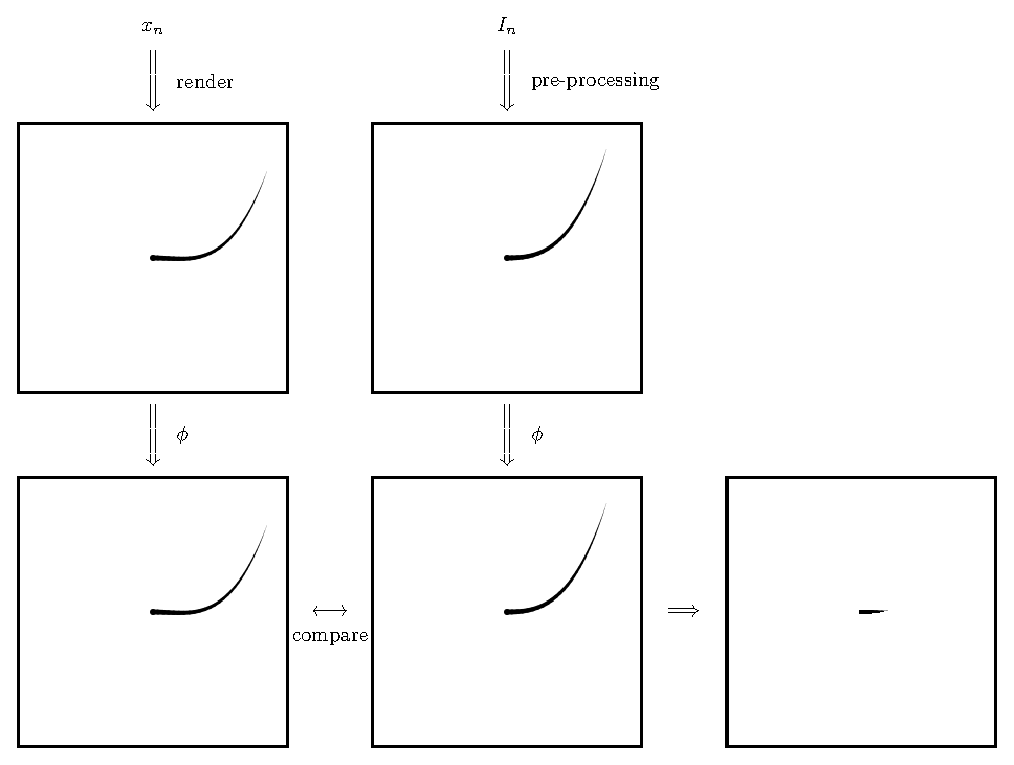
\includegraphics[scale=1.5]{whisker_compare.pdf}
\end{center}
